% !TEX root = ../thesis.tex

\section{Implementation}
\label{sec:implementation}
This is the Implementation.

\subsection{Groundwork: CataRT Extension}
\label{subsec:implementation_catart}
For the purpose of laying the groundwork for a bigger standalone application
(see section \ref{subsec:implementation_som-browser}), a proof-of-concept
implementation of the core \gls{som} algorithm was written in JavaScript to
serve as an extension to the \textit{MuBu For Max} software package
(\citet{web:mubu2019}, \citet{web:mubu2019_2}) for the visual programming
language Max \citep{web:max2019}. \textit{MuBu For Max} was developed by the
Sound, Music, Movement, Interaction Team (ISMM) at \gls{ircam}
\citep{schnell2009}. It contains the \textit{catart-by-mubu} patch for
realtime interactive corpus-based concatenative synthesis based on the original
\textit{CataRT} software \citep{schwarz2006}.


\begin{figure}[!htb]
  \centering
  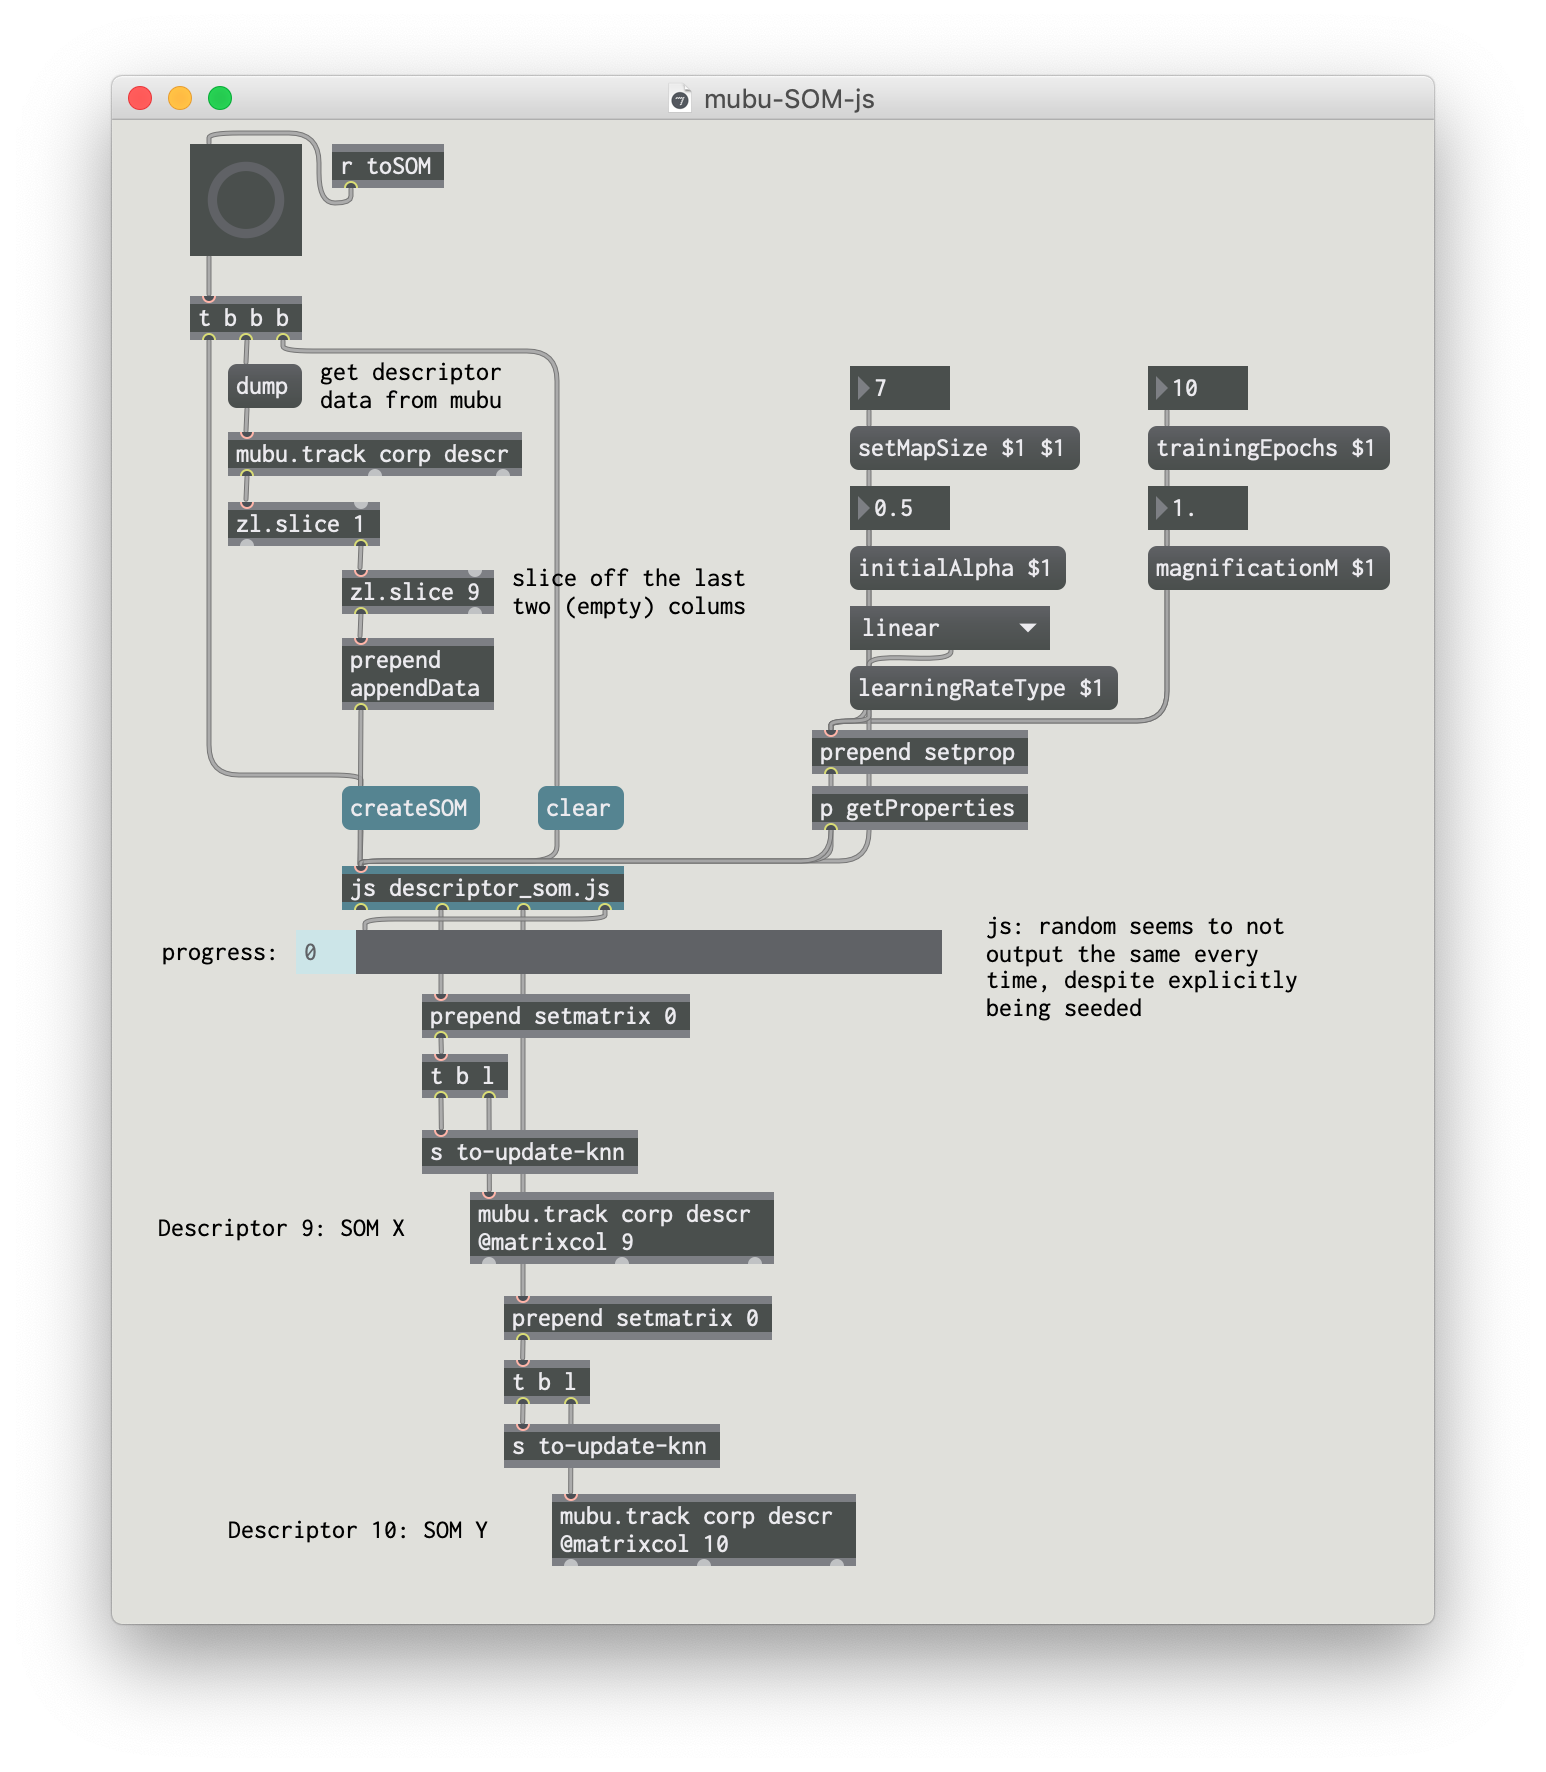
\includegraphics[width=\linewidth, clip]{mubu-som-js}
  \caption{mubu-SOM-js}
  \label{fig:mubu-som}
\end{figure}

\subsubsection{Functionality}
\label{subsubec:mubu-som_functionality}
\textit{Catart-by-mubu} uses a
two-dimensional scatter plot interface in which the user can select samples or
grains from the loaded audio corpus (see
% TODO
graphic here).
The spatial position of these sounds in the interface is determined by two audio
features, representing the horizontal and vertical axes, that can be selected by
the user.
The implemented \gls{som} extension gives users the option to choose a
two-dimensional \gls{som} for the spatial organization of the corpus. This is
augments the interface in three ways: all analyzed audio features can be
taken into account for the spatial positioning (as opposed to just two at a
time), more of the available interface space is used and additionally the sounds
are spaced in a more even fashion (see
% TODO
graphic here).

\textit{Mubu-SOM-js} offers the user simple controls to influence the produced
\gls{som}. These can be set by sending the following messages to the \\
\texttt{[js descriptor\_som.js]} object:

% TODO: make this a table???

\paragraph*{setMapSize} takes an integer value and sets the size of the square
map to that value.

\paragraph*{trainingEpochs} defines the length of the
training in epochs. One epoch corresponds to $n$ iterations of the training
algorithm as defined in section \ref{subsubsec:som_math_definition}, where $n$
is the number of samples in the corpus. Specified in integers.

\paragraph*{initialAlpha} is the starting value for $\alpha$, the learning rate
factor. It is expected to be a floating point value.

\paragraph*{learningRateType} sets the learning rate type (see section
\ref{subsubsec:som_learning_rates}). It expects a string that is either
\mintinline{js}{'linear'}, \mintinline{js}{'inverse'} or \mintinline{js}{'BDH'}.

\paragraph*{magnificationM} only applies when
\mintinline{js}{learningRateType === 'BDH'}. It expects a floating point value
and sets the magnification control factor $m$ (see section
\ref{para:alpha_bdh}).

\subsubsection{Code Overview}
\label{subsubsec:mubu-som_overview}

main training loop:

\begin{listing}[!htb]
  \begin{mdframed}
    \inputminted[breaklines, numbers=left, firstline=306, lastline=312,
    fontsize=\footnotesize]{js}{../dev/mubu-som-js/descriptor_som.js}
  \end{mdframed}
  \caption{mubu-som-js/descriptor\_som.js: neuron position updates inside
  \mintinline{js}{trainingStep()}}
\end{listing}

\subsection{SOM Browser}
\label{subsec:implementation_som-browser}

\subsubsection{Functionality}
\label{subsubsec:som-browser_functionality}
desired functionality

\subsubsection{Libraries and Frameworks Used}
\label{subsubsec:som-browser_libraries}

\paragraph{Electron}
\label{para:electron}

\paragraph{React}
\label{para:react}
reference boilerplate project

\paragraph{Web Audio API}
\label{para:web_audio_api}

\paragraph{Meyda}
\label{para:meyda}

choice of tools / frameworks:
- Electron
- React
- Web Audio (?)
- Meyda

what is application state?

\subsubsection{Application Structure}
\label{subsubsec:som-browser_structure}

Program structure:

\paragraph{System States}
\label{para:som-browser_states}
progression through system states

\paragraph{Background Processing}
\label{para:som-browser_background_processing}
background processing

\subsubsection{User Interface Components}
\label{subsubsec:som-browser_components}
App.js / components overview

\begin{listing}[!htb]
  \begin{mdframed}
    \inputminted[numbers=left, firstline=400, lastline=460,
    fontsize=\scriptsize]{jsx}{../dev/som-browser/src/components/App.js}
  \end{mdframed}
  \caption{som-browser/src/components/App.js:
  \mintinline{jsx}{<div className="AppContent">}}
  \label{lst:som-browser_app_content}
\end{listing}

\paragraph{TitleBar}
\label{para:title_bar}

\paragraph{MenuBar}
\label{para:menu_bar}

\paragraph{FileList}
\label{para:file_list}

\paragraph{Settings}
\label{para:settings}

\paragraph{Map}
\label{para:map}

\paragraph{FileInfo}
\label{para:file_info}

\paragraph{UserSelection}
\label{para:user_selection}

% TODO: FNP here???????
